\section {Frontend}
The following section describes the product the frontend team developed during the course.
The product consists of two different applications: Elephant, the web browser, and an implementation
of the NetInf services.

\subsection{Elephant Web Browser}
\label{sec:Elephant Web Browser}
The color of the spin-progress-bar indicates the medium used for fetching data.  
\begin{itemize}
\item Red indicates the uplink connection (3G or Wi-Fi)
\item Green indicates the database
\item Black indicates a NRS caching node
\item Blue indicates Bluetooth
\end{itemize}
Other than these colors, grey means that a search is currently in progress.
The application also offers the possibility to interrupt the
loading process by tapping on the the same icon used to start loading a page, as it toggles between a refresh
icon and cancel icon. 
\begin{figure}
\centering
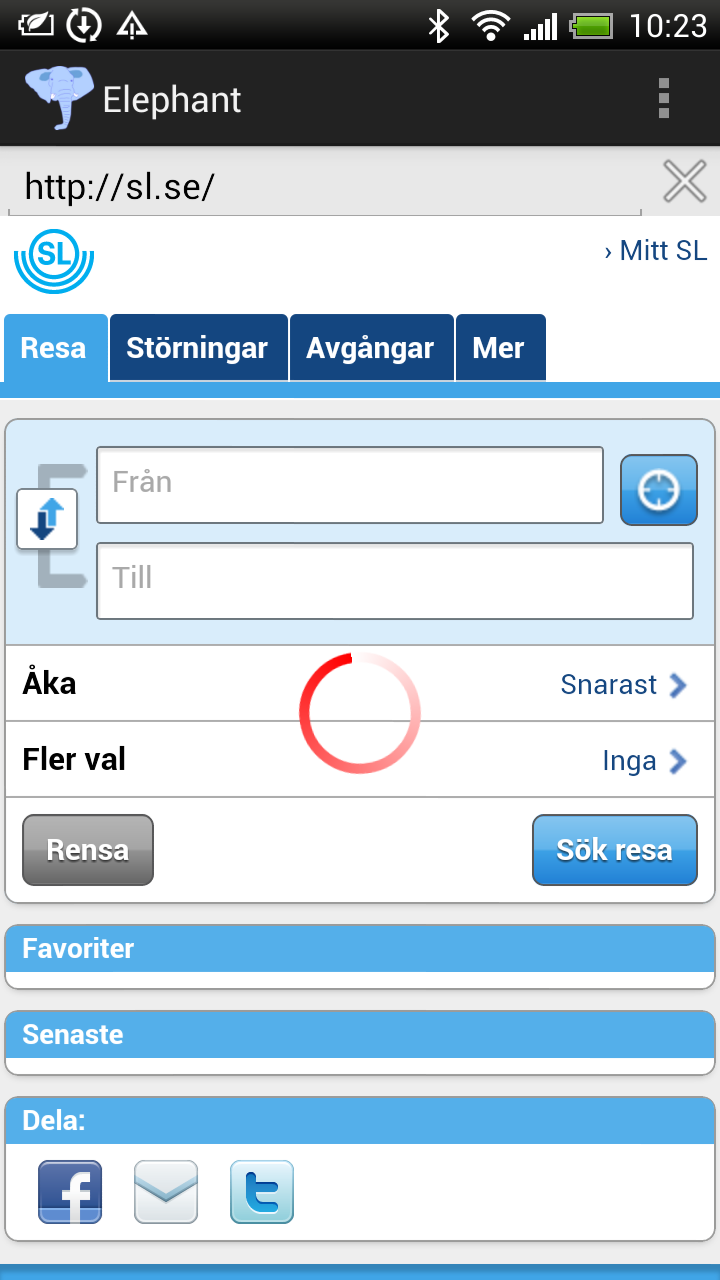
\includegraphics[scale=0.29]{img/loaded_page.png}
\caption{Loading a web page via uplink}\label{fig:loaded_page}
\end{figure}

\fig{loaded_page} shows an example view of the web browser.\\


To make sure that Elephant is able to retrieve resources from other mediums than the uplink, the NetInf service application must be up and running.
This is because the NetInf service enables communication to other nodes in the network and to keep track of which devices have a certain resource to serve via Bluetooth.

Elephant contains some customizable settings that can be found in the menu entry on the top right of the application.
These settings make it possible to take advantage of the NetInf service. In comparison to other
available browsers, Elephant makes use of Information-Centric Networking as well as Location-Based Networking
in an attempt to lower network congestion.
In the setting page, see \fig{ele_settings}, the user can decide if they want to share visited pages as well as upload web pages to a caching node.
The first menu entry gives the possibility to register the local device as a locator that can serve other devices via Bluetooth.
By enabling the second menu entry the device will not only register as a locator, but will also transfer the actual files to a NRS cache node, if any.

The last menu entry for the setting is for opening the NetInf Service's settings, so that the user does not have to switch applications
manually when changing the service settings.
\newpage

\begin{figure}
\centering
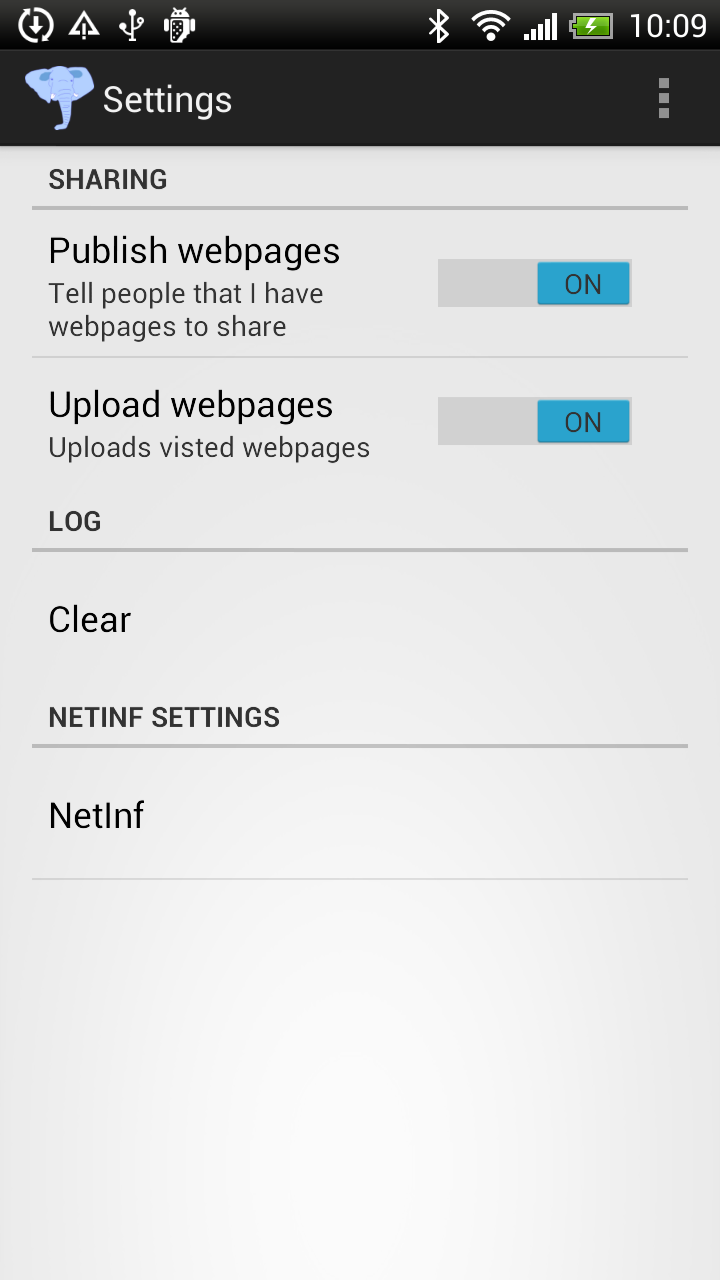
\includegraphics[scale=0.29]{img/ele_settings.png}
\caption{Settings view of Elephant}\label{fig:ele_settings}
\end{figure}

\newpage
Finally, \fig{help} shows a simple help view presenting a brief description of the functionalities of the application,
so that the user can have a better understanding of how the web browser works.\\

\begin{figure}
\centering
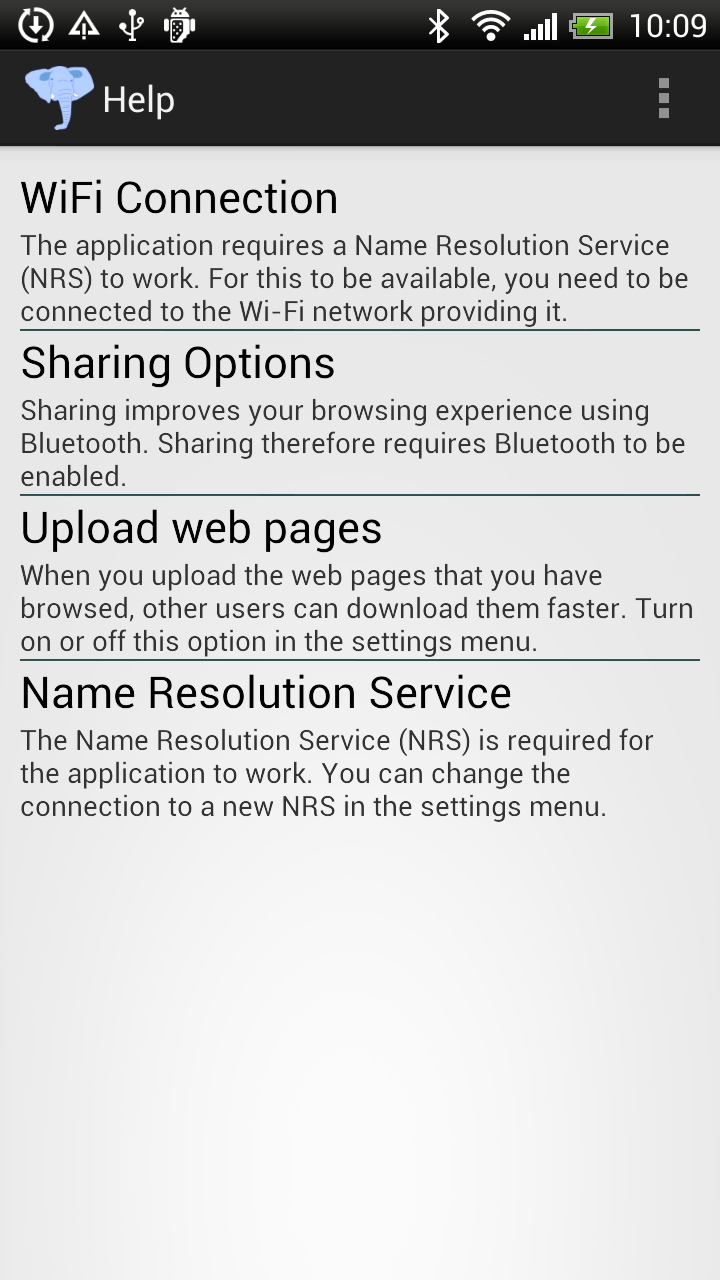
\includegraphics[scale=0.29]{img/help.png}
\caption{Help view}\label{fig:help}
\end{figure}

\subsection{NetInfService}

\begin{table}
\centering
 \begin{tabular}{|c|p{10cm}|}\hline
  Functionality	& Description \\\hline
  Search	& The application searches for the hash value of the resource requested, specified by a URL. This search includes
		  searching for the hash value within the local database and the remote Name Resolution Service (NRS).
		  It returns the value, if found.\\\hline
  Get		& A Get request that contains the hash value of an NDO triggers a content retrieval of the
		  corresponding resource. The application tries to retrieve the content either from the Local Resolution Service (LRS), the NRS
		  or from a remote Bluetooth device.\\\hline
  Publish	& The application can register the local device as a locator for a resource specified by a hash in the NRS. This way, remote
		  devices can try to retrieve that resource from the local device using Bluetooth. \\\hline
  Full put	& The full put is a publish request that contains the actual content corresponding to the resource that is published. Thus,
		  the NRS, to which the local device is connected to, can store the content and serve it itself.\\\hline
		  
 \end{tabular}
  \caption{Functionalities}\label{tab:netinffunctionalities}
\end{table}

The NetInfService is a stand-alone application that can be used by other
applications in order to make use of Information-Centric Networking. All functionalities
that are provided are listed in \tab{netinffunctionalities}. If an application
needs the ICN services, the NetInf Service application has to run in the background.\\

\begin{figure}
\centering
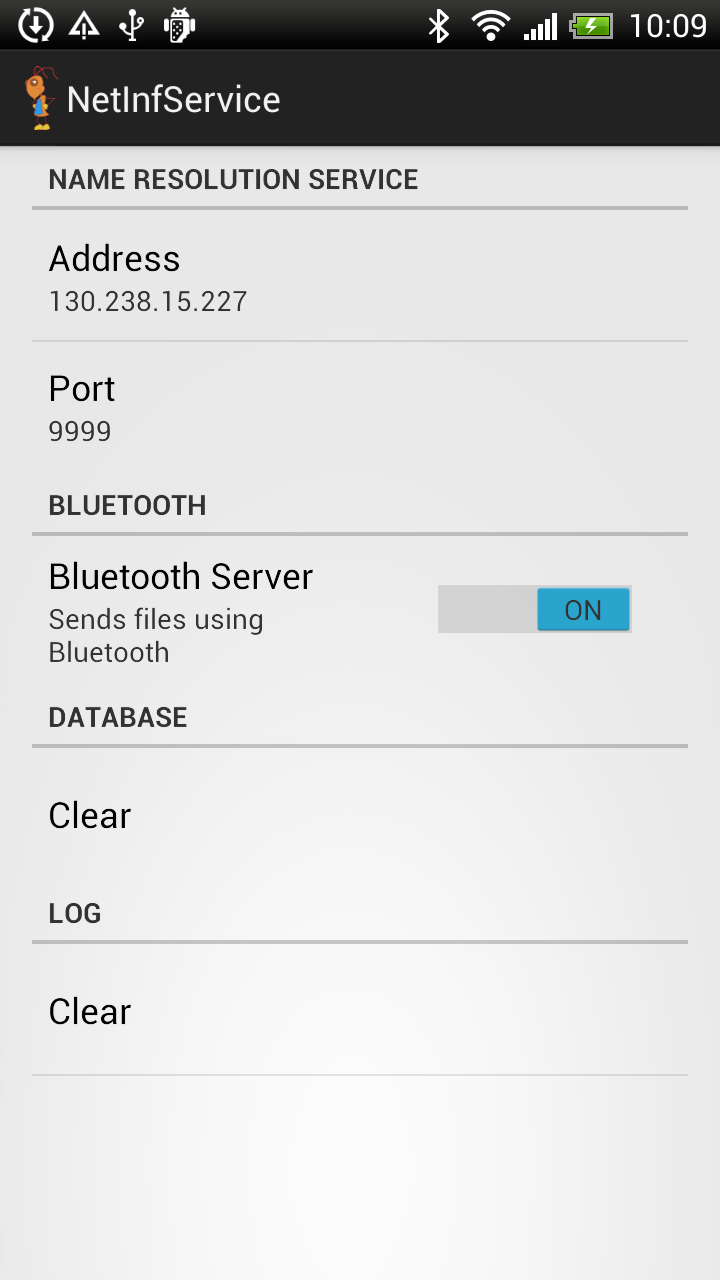
\includegraphics[scale=0.29]{img/ant_settings.png}
\caption{NetInf Service Settings}\label{fig:servicesettings}
\end{figure}

The services are configurable within a simple and self-explanatory user interface that is shown in \fig{servicesettings}.
If a user wants to change the NRS that the device is communicating with, the address as well as the port can be changed accordingly.
In addition a user can decide whether they want to share their downloaded content with other remote devices. Only if the \textit{Bluetooth Server} 
is turned on, data will be shared.
Finally, the database as well as the logs created during the run can be cleared.
The database stores every single resource that is published. At some point, the database will contain a huge amount of old data that is not
usable anymore. Clearing the database will then improve the run time since the search among stored content will perform faster.
Log files are used for debugging purposes. In case a log is old, clear it and rerun the application in order to 
gain new logs.
